%! TEX program = lualatex

% Use :VimtexToggleMain to compile this file alone with Vimtex
\documentclass[tikz]{standalone}

\usepackage{sty/adantikz}

\begin{document}
% Draw a series of rectangles for the optimal time-varying controller in the
% (q,p) plane
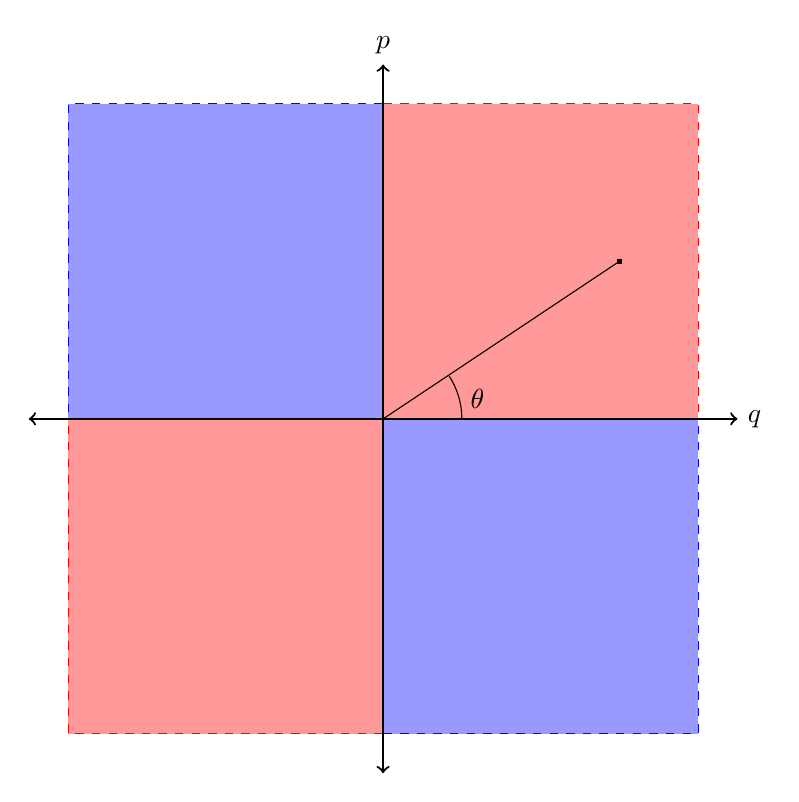
\begin{tikzpicture}
    % Fill each quadrant with a coloured rectangle, where red = standing and
    % blue = squatting
    \filldraw[fill=red!40,draw=red,dashed] (0,0) rectangle (4,4);
    \filldraw[fill=blue!40,draw=blue,dashed] (0,0) rectangle (-4,4);
    \filldraw[fill=red!40,draw=red,dashed] (0,0) rectangle (-4,-4);
    \filldraw[fill=blue!40,draw=blue,dashed] (0,0) rectangle (4,-4);
    % Draw the axes of the (q,p) plane on top of these rectangles
    \draw[draw=black,thick, <->] (-4.5,0) -- (4.5,0) node[right] {$q$};
    \draw[draw=black,thick, <->] (0,-4.5) -- (0,4.5) node[above] {$p$};
    % Draw an arc with the theta label up to some node in the plane
    \draw[draw=black] (0,0) -- (3,2) node[fill=black,inner sep= 1pt] {};
    \draw[draw = black] (1,0) arc (0:33:1) node at (1.2,0.25) {$\theta$};
\end{tikzpicture}
\end{document}
% vim: set tw=80 ts=4 sw=4 sts=0 et ffs=unix :
